\documentclass[../main/main.tex]{subfiles}

\begin{document}

\newpage

\chapter{Technical Solution}
\localtableofcontents

\section{File Tree Diagram}
To help navigate through the source code, I have included the following directory tree diagram, and put appropiate comments to explain the general purpose of code contained within specifc directories and Python files.

\begin{figure}[H]
    \centering
    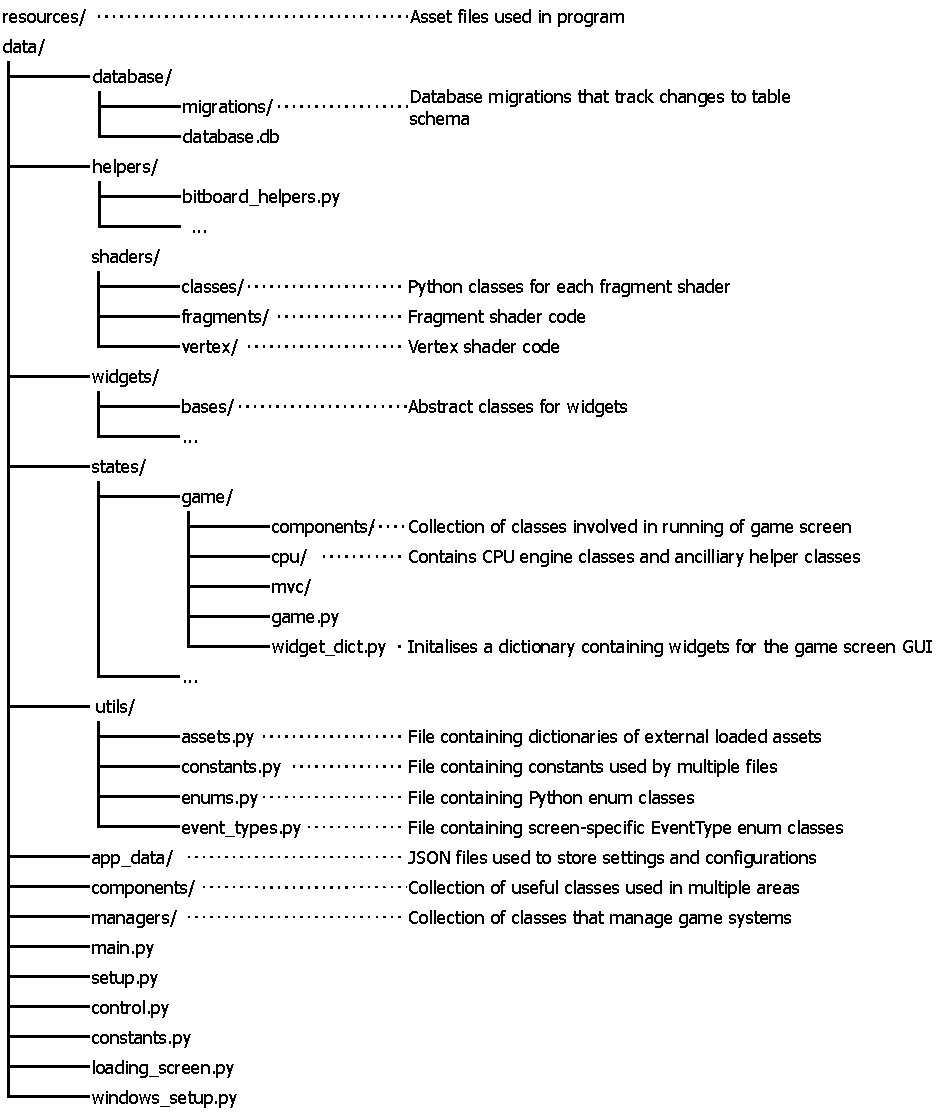
\includegraphics[width=\columnwidth]{../technical_solution/assets/file_tree_diagram.pdf}
    \caption{File tree diagram}
    \label{fig:file-tree-diagram}
\end{figure}

\section{Summary of Complexity}
\begin{itemize}
\item Alpha-beta pruning and transposition table improvements for Minimax (\ref{sec:alpha-beta} and \ref{sec:transposition-table})
\item Shadow mapping and coordinate transformations
\item Recursive Depth-First Search tree traversal (\ref{sec:theme} and \ref{sec:minimax})
\item Circular doubly-linked list and stack (\ref{sec:linked-list})
\item Multipass shaders and gaussian blur
\item Aggregate and Window SQL functions
\item OOP techniques (\ref{sec:widget-bases} and \ref{sec:widgets})
\item Multithreading (\ref{sec:loading-screen} and \ref{sec:cpu-thread})
\item Bitboards (\ref{sec:bitboards})
\item Zobrist hashing (\ref{sec:zobrist-hashing})
\item (File handling and JSON parsing) (\ref{sec:data-helpers})
\item (Dictionary recursion) (\ref{sec:theme})
\item (Dot product) (\ref{sec:asset-helpers})
\end{itemize}

\section{Overview}
\subsection{Main}
The file \lstinline{main.py} is run by the root file \lstinline{run.py}. Here resources-intensive classes such as the state and asset files are initialised, while the program displays a loading screen to hide the loading process. The main game loop is then executed.

\noindent\verb|main.py|
\lstinputlisting{../../data/main.py}

\subsection{Loading Screen}
\label{sec:loading-screen}
Multithreading is used to separate the loading screen GUI from the resources intensive actions in \lstinline{main.py}, to keep the GUI responsive. The easing function \lstinline{easeOutBack} is also used to animate the logo.

\noindent\verb|loading_screen.py|
\lstinputlisting{../../data/loading_screen.py}

\subsection{Helper functions}
These files provide useful functions for different classes.

\label{sec:asset-helpers}
\noindent\verb|asset_helpers.py (Functions used for assets and pygame Surfaces)|
\lstinputlisting{../../data/utils/asset_helpers.py}

\bigskip
\label{sec:data-helpers}
\noindent\verb|data_helpers.py (Functions used for file handling and JSON parsing)|
\lstinputlisting{../../data/utils/data_helpers.py}

\bigskip
\noindent\verb|widget_helpers.py (Files used for creating widgets)|
\lstinputlisting{../../data/utils/widget_helpers.py}

\subsection{Theme}
\label{sec:theme}
The theme manager file is responsible for providing an instance where the colour palette and dimensions for the GUI can be accessed.

\noindent\verb|theme.py|
\lstinputlisting{../../data/managers/theme.py}

\section{GUI}
\subsection{Laser}
The \lstinline{LaserDraw} class draws the laser in both the game and review screens.

\noindent\verb|laser_draw.py|
\lstinputlisting{../../data/states/game/components/laser_draw.py}

\subsection{Particles}
The \lstinline{ParticlesDraw} class draws particles in both the game and review screens. The particles are either fragmented pieces when destroyed, or laser particles emitted from the Sphinx. Particles are given custom velocity, rotation, opacity and size parameters.

\noindent\verb|particles_draw.py|
\lstinputlisting{../../data/states/game/components/particles_draw.py}

\subsection{Widget Bases}
\label{sec:widget-bases}
Widget bases are the base classes for for my widgets system. They contain both attributes and getter methods that provide basic functionality such as size and position, and abstract methods to be overriden. These bases are also designed to be used with multiple inheritance, where multiple bases can be combined to add functionality to the final widget. Encapsulation also allows me to simplify interactions between widgets, as using getter methods instead of protected attributes allows me to add logic while accessing an attribute, such as in \verb|widget.py|, where the logic to fetch the parent surface instead of the windows screen is hidden within the base class.

\bigskip
\noindent All widgets are a subclass of the \lstinline{Widget} class.

\noindent\verb|widget.py|
\lstinputlisting{../../data/widgets/bases/widget.py}

\bigskip
\noindent The \lstinline{Circular} class provides functionality to support widgets which rotate between text/icons.
\noindent\verb|circular.py|
\lstinputlisting{../../data/widgets/bases/circular.py}

\subsubsection{Circular Linked List}
\label{sec:linked-list}
The \lstinline{CircuarLinkedList} class implements a circular doubly-linked list. Used for the internal logic of the \lstinline{Circular} class.

\noindent\verb|circular_linked_list.py|
\lstinputlisting{../../data/components/circular_linked_list.py}

\subsection{Widgets}
\label{sec:widgets}
Each state contains a \lstinline{WIDGET_DICT} map, which contains and initialises each widget with their own attributes, and provides references to run methods on them in the state code. Each \lstinline{WIDGET_DICT} is passed into a \lstinline{WidgetGroup} object, which is responsible for drawing, resizing and handling all widgets for the current state.

The \lstinline{CustomEvent} class is used to pass data between states and widgets. An event argument is passed into interactive widgets; When a widget wants to pass data back to the state, it returns the event, and adds any attributes that is required. The state then receives and handles these returned events accordingly.

\noindent\verb|custom_event.py|
\lstinputlisting{../../data/components/custom_event.py}

Below is a list of all the widgets I have implemented:

\begin{multicols}{3}
\begin{itemize}
\item BoardThumbnailButton
\item MultipleIconButton
\item ReactiveIconButton
\item BoardThumbnail
\item ReactiveButton
\item VolumeSlider
\item ColourPicker
\item ColourButton
\item BrowserStrip
\item PieceDisplay
\item BrowserItem
\item TextButton
\item IconButton
\item ScrollArea
\item Chessboard
\item TextInput
\item Rectangle
\item MoveList
\item Dropdown
\item Carousel
\item Switch
\item Timer
\item Text
\item Icon
\item (\_ColourDisplay)
\item (\_ColourSquare)
\item (\_ColourSlider)
\item (\_SliderThumb)
\item (\_Scrollbar)
\end{itemize}
\end{multicols}

\bigskip
\noindent The \lstinline{ReactiveIconButton} widget is a pressable button that changes the icon displayed when it is hovered or pressed.

\noindent\verb|reactive_icon_button.py|
\lstinputlisting{../../data/widgets/reactive_icon_button.py}

\bigskip
\noindent The \lstinline{ReactiveButton} widget is the parent class for \lstinline{ReactiveIconButton}. It provides the methods for clicking, rotating between widget states, positioning etc.

\noindent\verb|reactive_button.py|
\lstinputlisting{../../data/widgets/reactive_button.py}

\bigskip
\noindent The \lstinline{ColourSlider} widget is instanced in the \lstinline{ColourPicker} class. It provides a slider for changing between hues for the colour picker, using the functionality of the \lstinline{SliderThumb} class.

\noindent\verb|colour_slider.py|
\lstinputlisting{../../data/widgets/colour_slider.py}

\bigskip
\noindent The \lstinline{TextInput} widget is used for inputting fen strings and time controls.

\noindent\verb|text_input.py|
\lstinputlisting{../../data/widgets/text_input.py}

\section{Game}
\subsection{Model}
\noindent\verb|game_model.py|
\lstinputlisting{../../data/states/game/mvc/game_model.py}

\subsection{View}
\noindent\verb|game_view.py|
\lstinputlisting{../../data/states/game/mvc/game_view.py}

\subsection{Controller}
\noindent\verb|game_controller.py|
\lstinputlisting{../../data/states/game/mvc/game_controller.py}

\subsection{Board}
The \lstinline{Board} class implements the Laser Chess board, and is responsible for handling moves, captures, and win conditions.

\noindent\verb|board.py|
\lstinputlisting{../../data/states/game/components/board.py}

\subsection{Bitboards}
\label{sec:bitboards}
The \lstinline{BitboardCollection} class uses helper functions found in \lstinline{bitboard_helpers.py} such as \lstinline{pop_count}, to initialise and manage bitboard transformations.

\noindent\verb|bitboard_collection.py|
\lstinputlisting{../../data/states/game/components/bitboard_collection.py}

\section{CPU}
This section includes my implementation for the CPU engine run on minimax, including its various improvements and accessory classes.

Every CPU engine class is a subclass of a \lstinline{BaseCPU} abstract class, and therefore contains the same attribute and method names. This means polymorphism can be used again to easily to test and vary the difficulty by switching out which CPU engine is used.

The method \lstinline{find_move} is called by the CPU thread. \lstinline{search} is then called recursively to traverse the minimax tree, and find an optimal move. The move is then return to \lstinline{find_move} and passed and run with the callback function.

\subsection{Minimax}
\label{sec:minimax}
\noindent\verb|minimax.py|
\lstinputlisting{../../data/states/game/cpu/engines/minimax.py}

\subsection{Alpha-beta Pruning}
\label{sec:alpha-beta}
\noindent\verb|alpha_beta.py|
\lstinputlisting[lastline=94]{../../data/states/game/cpu/engines/alpha_beta.py}

\subsection{Transposition Table}
\label{sec:transposition-table}
For adding transposition table functionality to my other engine classes, I have decided to use a mixin design architecture. This allows me to reuse code by adding mixins to many different classes, and inject additional transposition table methods and functionality into other engines.

\noindent\verb|transposition_table.py|
\lstinputlisting[lastline=59]{../../data/states/game/cpu/engines/transposition_table.py}

\subsection{Evaluator}
\noindent\verb|evaluator.py|
\lstinputlisting{../../data/states/game/cpu/evaluator.py}

\subsection{Multithreading}
A \lstinline{CPUThread} is initialised with a CPU engine at the start of the game state, and run whenever it is the CPU's turn to move.

\noindent\verb|cpu_thread.py|
\label{sec:cpu-thread}
\lstinputlisting{../../data/states/game/cpu/cpu_thread.py}

\subsection{Zobrist Hashing}
\label{sec:zobrist-hashing}
\noindent\verb|zobrist_hasher.py|
\lstinputlisting{../../data/states/game/cpu/zobrist_hasher.py}

\subsection{Cache}
\noindent\verb|transposition_table.py|
\lstinputlisting{../../data/states/game/cpu/transposition_table.py}

\section{Database}
This section outlines my database implementation using Python sqlite3.

\subsection{DDL}
As mentioned in Section \ref{sec:design-ddl}, the \lstinline{migrations} directory contains a collection of Python scripts that edit the game table schema. The files are named with their changes and datetime labelled for organisational purposes.

\noindent\verb|create_games_table_19112024.py|
\lstinputlisting{../../data/database/migrations/create_games_table_19112024.py}
Using the \lstinline{ALTER} command allows me to rename table columns.

\bigskip
\noindent\verb|change_fen_string_column_name_23122024.py|
\lstinputlisting{../../data/database/migrations/change_fen_string_column_name_23122024.py}

\subsection{DML}
\noindent\verb|database_helpers.py|
\lstinputlisting{../../data/utils/database_helpers.py}

\section{Shaders}
\subsection{Shader Manager}
The \lstinline{ShaderManager} class is responsible for handling all shader passes, handling the Pygame display, and combining both and drawing the result to the window screen. The class also inherits from the \lstinline{SMProtocol} class, an interface class containing all required \lstinline{ShaderManager} methods and attributes to aid with syntax highlighting in the fragment shader classes.

\noindent\verb|shader.py|
\lstinputlisting{../../data/managers/shader.py}

\subsection{Rays}
\noindent\verb|occlusion.frag|
\lstinputlisting{../../data/shaders/fragments/occlusion.frag}

\bigskip
\noindent\verb|shadowmap.frag|
\lstinputlisting{../../data/shaders/fragments/shadowmap.frag}

\bigskip
\noindent\verb|lightmap.frag|
\lstinputlisting{../../data/shaders/fragments/lightmap.frag}

\subsection{Bloom}
\noindent\verb|highlight_colour.frag|
\lstinputlisting{../../data/shaders/fragments/highlight_colour.frag}

\noindent\verb|blur.frag|
\lstinputlisting{../../data/shaders/fragments/blur.frag}

\bigskip
\noindent\verb|blur.frag|
\lstinputlisting{../../data/shaders/fragments/blur.frag}

\subsection{Stack}


\end{document}